%% bare_jrnl.tex
%% V1.3
%% 2007/01/11
%% by Michael Shell
%% see http://www.michaelshell.org/
%% for current contact information.
%%
%% This is a skeleton file demonstrating the use of IEEEtran.cls
%% (requires IEEEtran.cls version 1.7 or later) with an IEEE journal paper.
%%
%% Support sites:
%% http://www.michaelshell.org/tex/ieeetran/
%% http://www.ctan.org/tex-archive/macros/latex/contrib/IEEEtran/
%% and
%% http://www.ieee.org/



% *** Authors should verify (and, if needed, correct) their LaTeX system  ***
% *** with the testflow diagnostic prior to trusting their LaTeX platform ***
% *** with production work. IEEE's font choices can trigger bugs that do  ***
% *** not appear when using other class files.                            ***
% The testflow support page is at:
% http://www.michaelshell.org/tex/testflow/


%%*************************************************************************
%% Legal Notice:
%% This code is offered as-is without any warranty either expressed or
%% implied; without even the implied warranty of MERCHANTABILITY or
%% FITNESS FOR A PARTICULAR PURPOSE! 
%% User assumes all risk.
%% In no event shall IEEE or any contributor to this code be liable for
%% any damages or losses, including, but not limited to, incidental,
%% consequential, or any other damages, resulting from the use or misuse
%% of any information contained here.
%%
%% All comments are the opinions of their respective authors and are not
%% necessarily endorsed by the IEEE.
%%
%% This work is distributed under the LaTeX Project Public License (LPPL)
%% ( http://www.latex-project.org/ ) version 1.3, and may be freely used,
%% distributed and modified. A copy of the LPPL, version 1.3, is included
%% in the base LaTeX documentation of all distributions of LaTeX released
%% 2003/12/01 or later.
%% Retain all contribution notices and credits.
%% ** Modified files should be clearly indicated as such, including  **
%% ** renaming them and changing author support contact information. **
%%
%% File list of work: IEEEtran.cls, IEEEtran_HOWTO.pdf, bare_adv.tex,
%%                    bare_conf.tex, bare_jrnl.tex, bare_jrnl_compsoc.tex
%%*************************************************************************

% Note that the a4paper option is mainly intended so that authors in
% countries using A4 can easily print to A4 and see how their papers will
% look in print - the typesetting of the document will not typically be
% affected with changes in paper size (but the bottom and side margins will).
% Use the testflow package mentioned above to verify correct handling of
% both paper sizes by the user's LaTeX system.
%
% Also note that the "draftcls" or "draftclsnofoot", not "draft", option
% should be used if it is desired that the figures are to be displayed in
% draft mode.
%
\documentclass{IEEEtran}
\usepackage{filecontents}
\usepackage{lipsum}
\usepackage[utf8]{inputenc}
\usepackage{graphicx} % for image

% correct bad hyphenation here
\hyphenation{op-tical net-works semi-conduc-tor}


\begin{document}
%
% paper title
% can use linebreaks \\ within to get better formatting as desired
\title{Estimador de Estado de Sistemas de Distribuição de Energia Utilizando Abordagem por Redes Neurais Artificiais com Número de Medições Reduzido}
%
%
% author names and IEEE memberships
% note positions of commas and nonbreaking spaces ( ~ ) LaTeX will not break
% a structure at a ~ so this keeps an author's name from being broken across
% two lines.
% use \thanks{} to gain access to the first footnote area
% a separate \thanks must be used for each paragraph as LaTeX2e's \thanks
% was not built to handle multiple paragraphs
%

\author{Luiz~Le~Roy,~\IEEEmembership{PUC Minas}
        % <-this % stops a space
\thanks{Texto finalizado em 15 de fevereiro de 2014.}}

% The paper headers
\markboth{Journal of \LaTeX\,~Vol.~X, No.~Y, Fevereiro~2014}%
{Shell \MakeLowercase{\textit{et al.}}: Bare Demo of IEEEtran.cls for Journals}

% make the title area
\maketitle

\begin{abstract}
%\boldmath
O artigo apresenta uma forma alternativa de modelagem para um estimador de estado de sistemas de distribuição (DSSE - Distribution System State Estimation). A partir de um determinado perfil de carga e medições reais o estado do sistema é gerado com auxílio de uma rede neural artificial (ANNs - Artificial Neuaral Networks).
O erro associado é utilizado para treinamento da rede através de minimização por um algoritmo evolucionário, denomidado PSO - \textit{Particle Swarm Optimiztion}. Originalmente (na principal referência deste trabalho), a otimização é utilizada através de mínimos quadrados ponderados (\textit{WLS - Weighted Least Squares}). Utiliza-se a decomposição em diversos componentes através do ``modelo de mistura gaussiano'' (GMM - Gaussian Mixture Model). No artigo do trabalho original, ``Distribution System State Estimation Using an Artificial Neural Network Approach for Pseudo Measurement Modeling'' de Manitsas et all (2012), o resultado do trabalho é demonstrado em um sistema de 95 barras do Reino Unido (U.K Generic Distribution System - UKGDS). Neste trabalho utiliza-se uma rede da Compania Energética de Minas Gerais - Cemig, fornecida por sua subsidiária Cemig Distribuição S.A.
\end{abstract}

\begin{IEEEkeywords}
Sistemas de Distribuição de Energia Elétrica, DSSE, ANNs, PSO, WLS, GMM.
\end{IEEEkeywords}

\IEEEpeerreviewmaketitle

\section{Introdução}
\IEEEPARstart{P}{ara} este trabalho, a principal referência foi o artigo \cite{manitsas2012distribution}. É possível constatar que o Estimador de Estado de Sistemas de Distribuição (Distribution System State Estimation - DSEE), eventualmente, não é uma ferramenta que providencia um resultado satisfatório a partir de um número limitado de medições. 

Quando o objetivo é tratar redes de distribuição de energia, diferentemente de redes de transmissão, os requisitos mínimos de redundância de informação podem não ser atingidos com um estimador de estados tradicional. Vários algoritmos têm sido sugeridos para estimar estado em \cite{schweppe1970powerI}, \cite{schweppe1970powerII}, \cite{schweppe1970powerIII}, \cite{abur2004power} e \cite{monticelli2000electric}. Todos estes algoritmos trabalham bem porque existe alta redundância nas medições. No entanto, em sistemas de distribuição, devido à alta dispersão das medições, existe menos ou nenhuma redundância. Por isso, quando estes algoritmos são expostos a sistemas de distribuição eles começam a mostrar suas limitações. Por exemplo, em sistemas de transmissão, estimador por mínimo valor absoluto ponderado (Weighted Least Absolute Value - WLAV) elimina dados ruins por medições redundantes, mas em sistemas de distribuição não. No trabalho original apresenta-se uma forma de providenciar uma estimativa rasoável do estado do sistema utilizando um número muito limitado de medidas.

Primeiramente, uma eficiente forma de modelar pseudo-medidas é expressá-las como uma função não linear. Partindo de medidas avaliadas nos principais pontos, e também localizadas nos locais de geração distribuída. Em sistemas pequenos, esta função pode  ser facilmente obtida pela curva típica do problema. Em grandes sistemas, o usual é utilizar uma abordagem através de redes neurais artificiais.

No artigo, uma rede neural artificial apropriada para modelar a potência ativa e reativa em um estimador de estados de sistemas de distribuição é apresentada. O perfil de carga e um reduzido número de de medições no fluxo de potência derivados de simulações é utilizado para treinar a rede. O erro entre a potência de entrada e o valor de saída da rede é modelado via GMM (Gaussian Mixture Model).

\section{Estimador de Estados}
O emprego do algoritmo WLS (\textit{Weighted Least Squares}) para o estimador de estado em redes de distribuição utilizando ``medidas padrão'' é utilizado em \cite{singh2009choice}. WLS é baseada na minimização da seguinte função objetivo (\ref{ffo}):
\begin{equation} \label{ffo}
J'=[\textbf{z}-\textbf{h}(\textbf{x})]^T\textbf{R}_z^{-1}[\textbf{z}-\textbf{h}(\textbf{x})]  
\end{equation}
Onde \textbf{z} e \textbf{x} são os vetores de medição e de componentes de estado respectivamente. Assume-se que estes vetores são relacionados pela equação $\textbf{z}=\textbf{h}(\textbf{x})+\textbf{e}_z$, onde $\textbf{h}(\textbf{x})$ é uma função conhecida. O vetor de erro de medida $\textbf{e}_z$ é assumido como uma variável randômica gaussiana com matriz de covariância $\textbf{R}_z=diag\{\sigma^2_{z1},\sigma^2_{z2}, ...,\sigma^2_{zm}\}$, i.e., a relação cruzada entre o erro de medida \cite{caro2009power} não é levado em consideração. Assim, $\sigma^2_{zi}$ é a variância da i-ésima medida.

Para este trabalho uma nova metodologia é proposta. A ideia é utilizar a capacidade de redes do tipo lógica (\cite{pedrycz2006or} e \cite{eu2014RNALogica}) no treinamento e minimizar a função objetivo da Eq. \ref{ffo} via PSO (\cite{del2008particle}).


\section{Redes Neurais Artificiais} \label{rna}
Uma ANN (\textit{Artificial Neural Network}) é um modelo que se baseia na arquitetura e funcionalidades das redes neurais \emph{\textbf{\textit{\textsl{\texttt{\textsc{biológica (\cite{manitsas2012distribution})}}}}}}. Elas são comumente utilizadas para análise de regressão e classificação. Bem como vários outros modelos de processamento de dados. Sua unidade de construção elementar é o neurônio. Recebe um número de entradas, processa, e gera uma outra quantidade de saídas. As entradas são combinadas linearmente através de pesos pré-calculados e utiliza-se uma função de transferência (conforme \cite{hippert2001neural}) para obter a saída da rede.

Nas ANNs do artigo original utiliza-se a técnica \textit{feed-forward} de duas camadas. 
%como mostrado na fig . 2 , 
Os neurônios são organizados em duas camadas, uma escondida , isto é, exite algo entre os nós de entrada e a camada de saída. A ANN é designada como \textit{feed-forward} quando as saídas de uma camada são as entradas para a próxima camada oculta. Utiliza-se funções de transferência sigmoide. As camada coincidem com o número de entradas necessárias para estimar o estado.

\section{Resultados}
Para fins didáticos, e de comparação, os principais resultados do artigo original são resumidos nas figuras e comentários abaixo.

A estrutura original é composta por uma rede de distribuição de energia elétrica do Reino Unido, onde não foi possível obter a data original de configuração. Mas a topologia é representada pela Fig. \ref{top_uk}.

\begin{figure}
	\centering
	\includegraphics{topologia_UK.pdf}
	\caption{Rede de teste UK (original)}
	\label{top_uk}
\end{figure}

Por dificuldades de se encontrar valores de ligação do circuito, cargas distribuídas e impedâncias de linha do modelo supracitado optou-se neste trabalho por utilizar uma rede similar à \textbf{topologia de rede que ocorre na prática aos sistema de distribuição de energia do estado de Minas Gerais (alimentadores longos com número grande de cargas distribuídas).} Uma destas redes é representada na figura \ref{top}.

\begin{figure*}
\centering
\includegraphics[width=155mm]{axxxx-05.pdf}
\caption{Perfil topológico do alimentador com a ligação entre as barras e a localização de todos os capacitores alocados destacada no retângulo.}
\label{top}
\end{figure*}

A rede para a primeira versão da rotina de cálculo é representada em \ref{top_moc}.

\begin{figure}
	\centering
	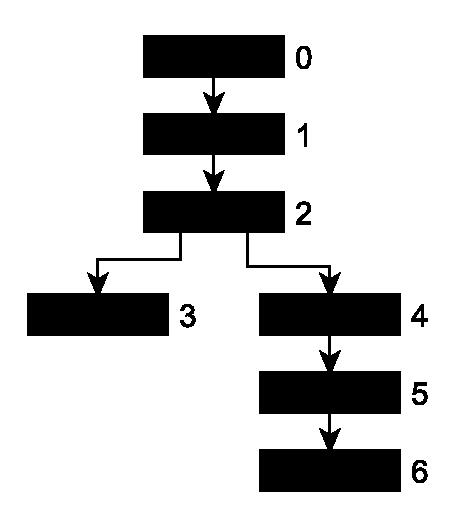
\includegraphics[width=50mm]{rede_moc.pdf}
	\caption{Rede de teste minimizada}
	\label{top_moc}
\end{figure}

Para esta estrutura o algoritmo original foi capaz de obter bons resultados no que tange o valor absoluto da tensão de saída.
\emph{\textbf{\textit{\textsl{\texttt{\textsc{Considerar falar sobre os resultados ruins em relação ao ângulo.}}}}}}

Pode-se observar a variação nos resultados do algoritmo através dos gráficos abaixo (Figs. 8-12 de Fig. \ref{topologia_full}).
\begin{figure*}
	\centering
	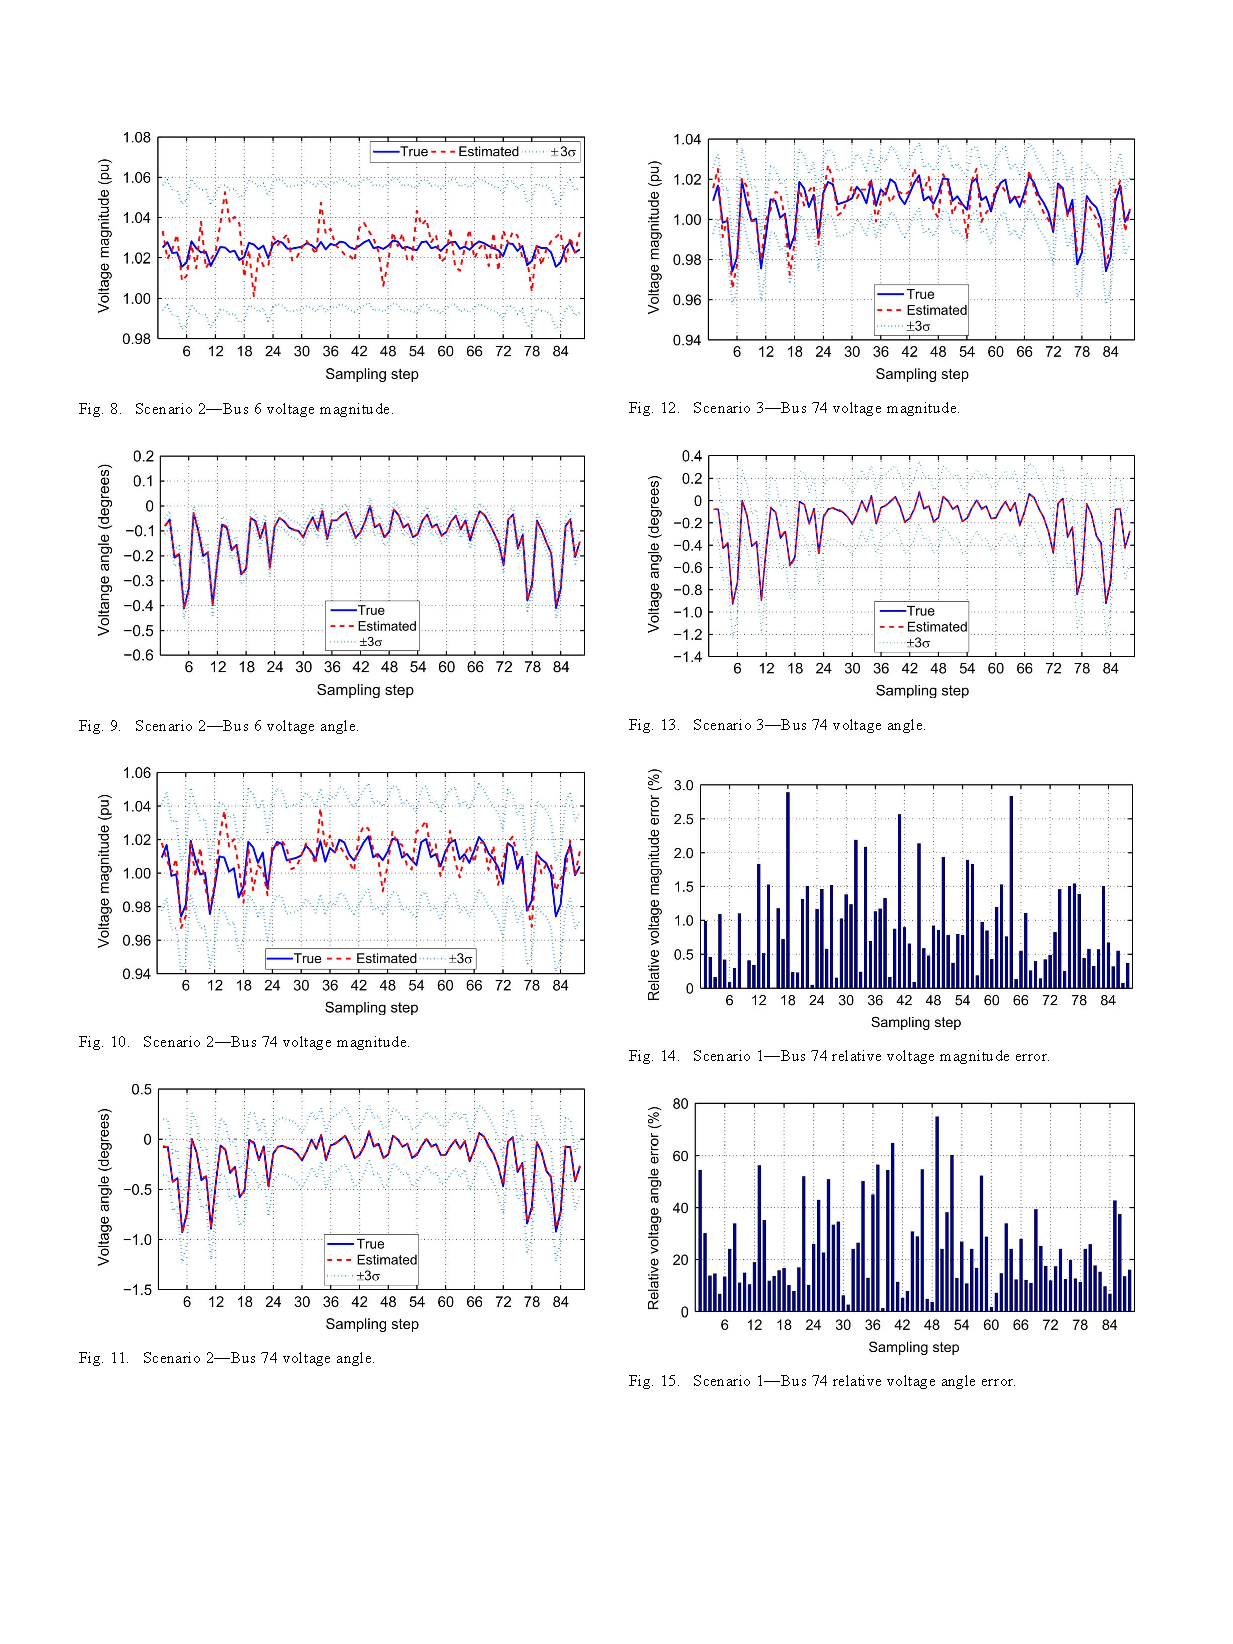
\includegraphics{topologia_full.pdf}
	\caption{Resultados originais: gráficos do artigo da primeira referência do trabalho}
	\label{topologia_full}
\end{figure*}

\section{Conclusão}
\textit{No fim deste trabalho segue a implementação, para discussão em sala.}
\begin{figure*}
	\centering
	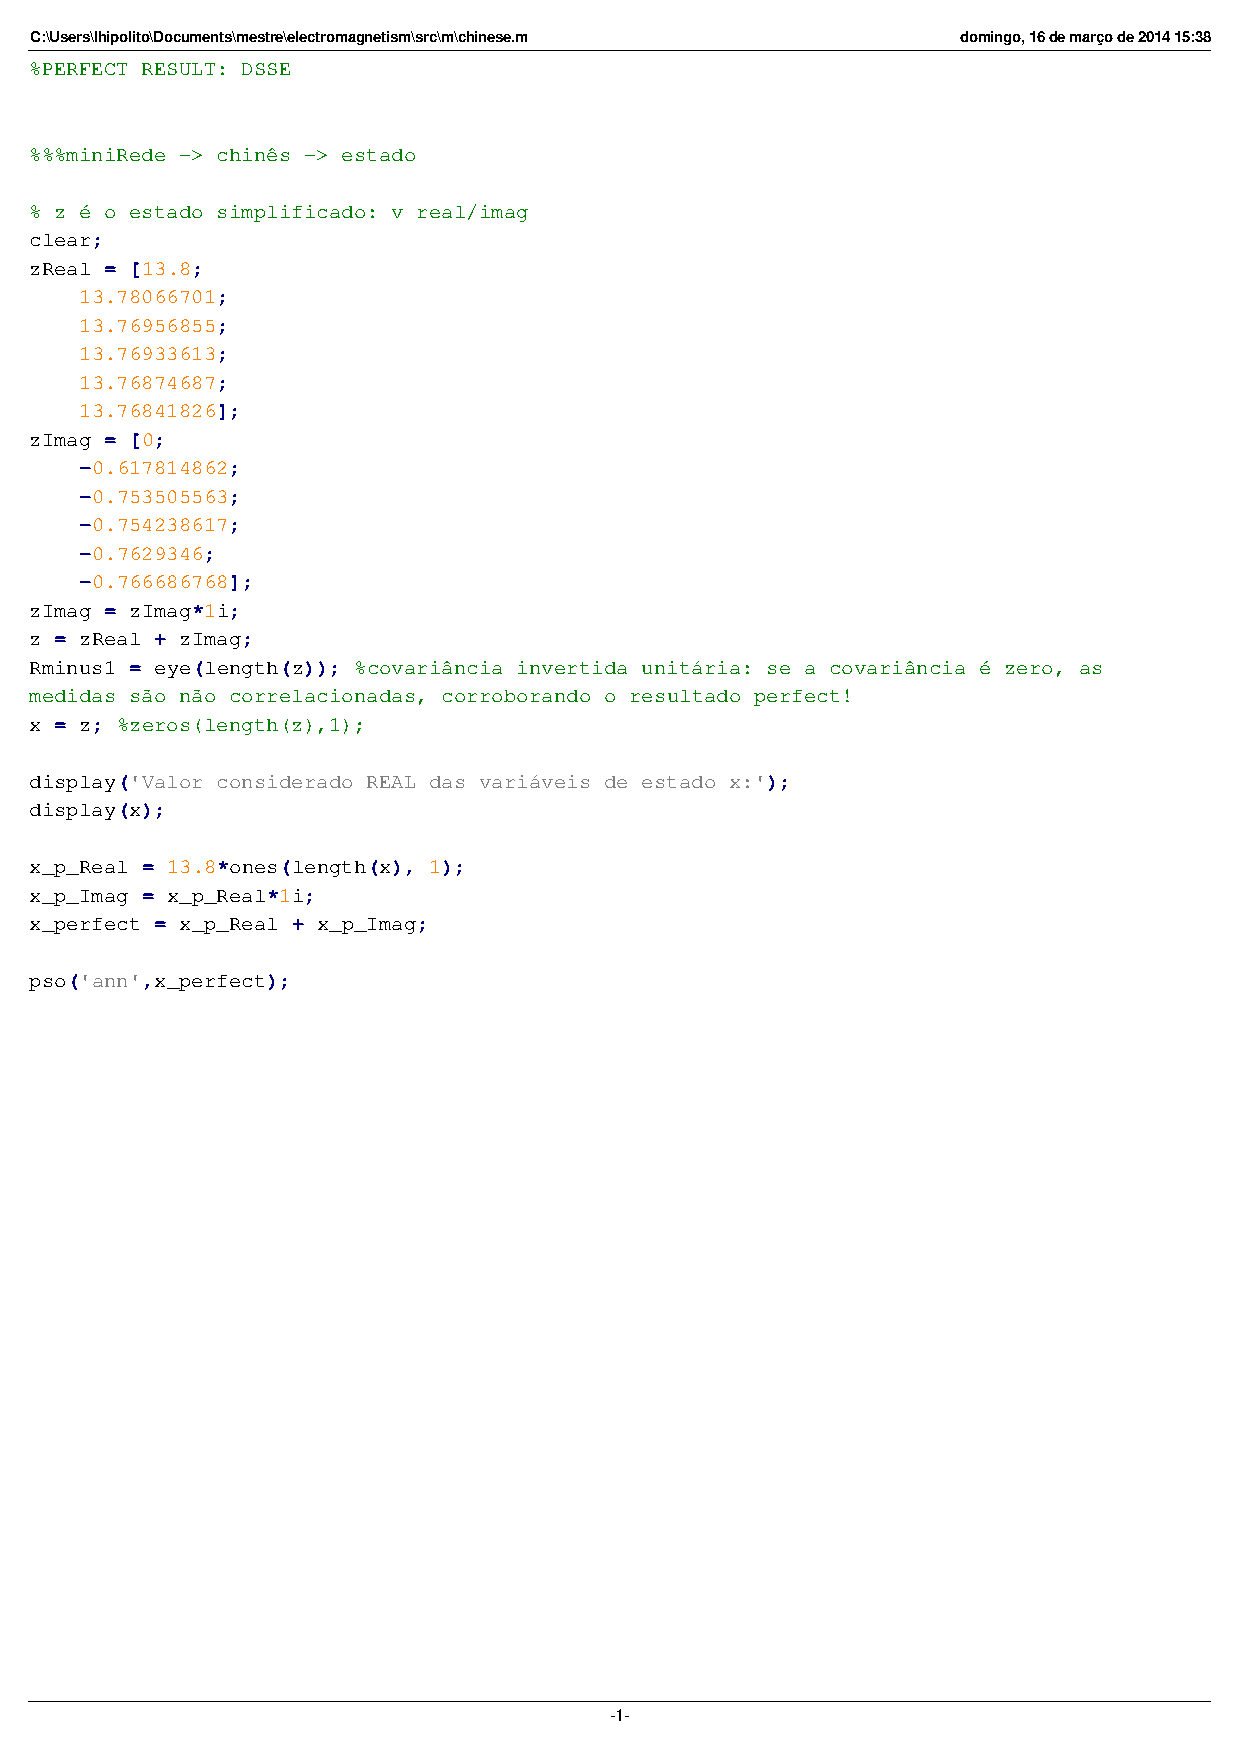
\includegraphics{chinese.pdf}
	%\caption{Código}
	\label{chinese}
\end{figure*}
\begin{figure*}
	\centering
	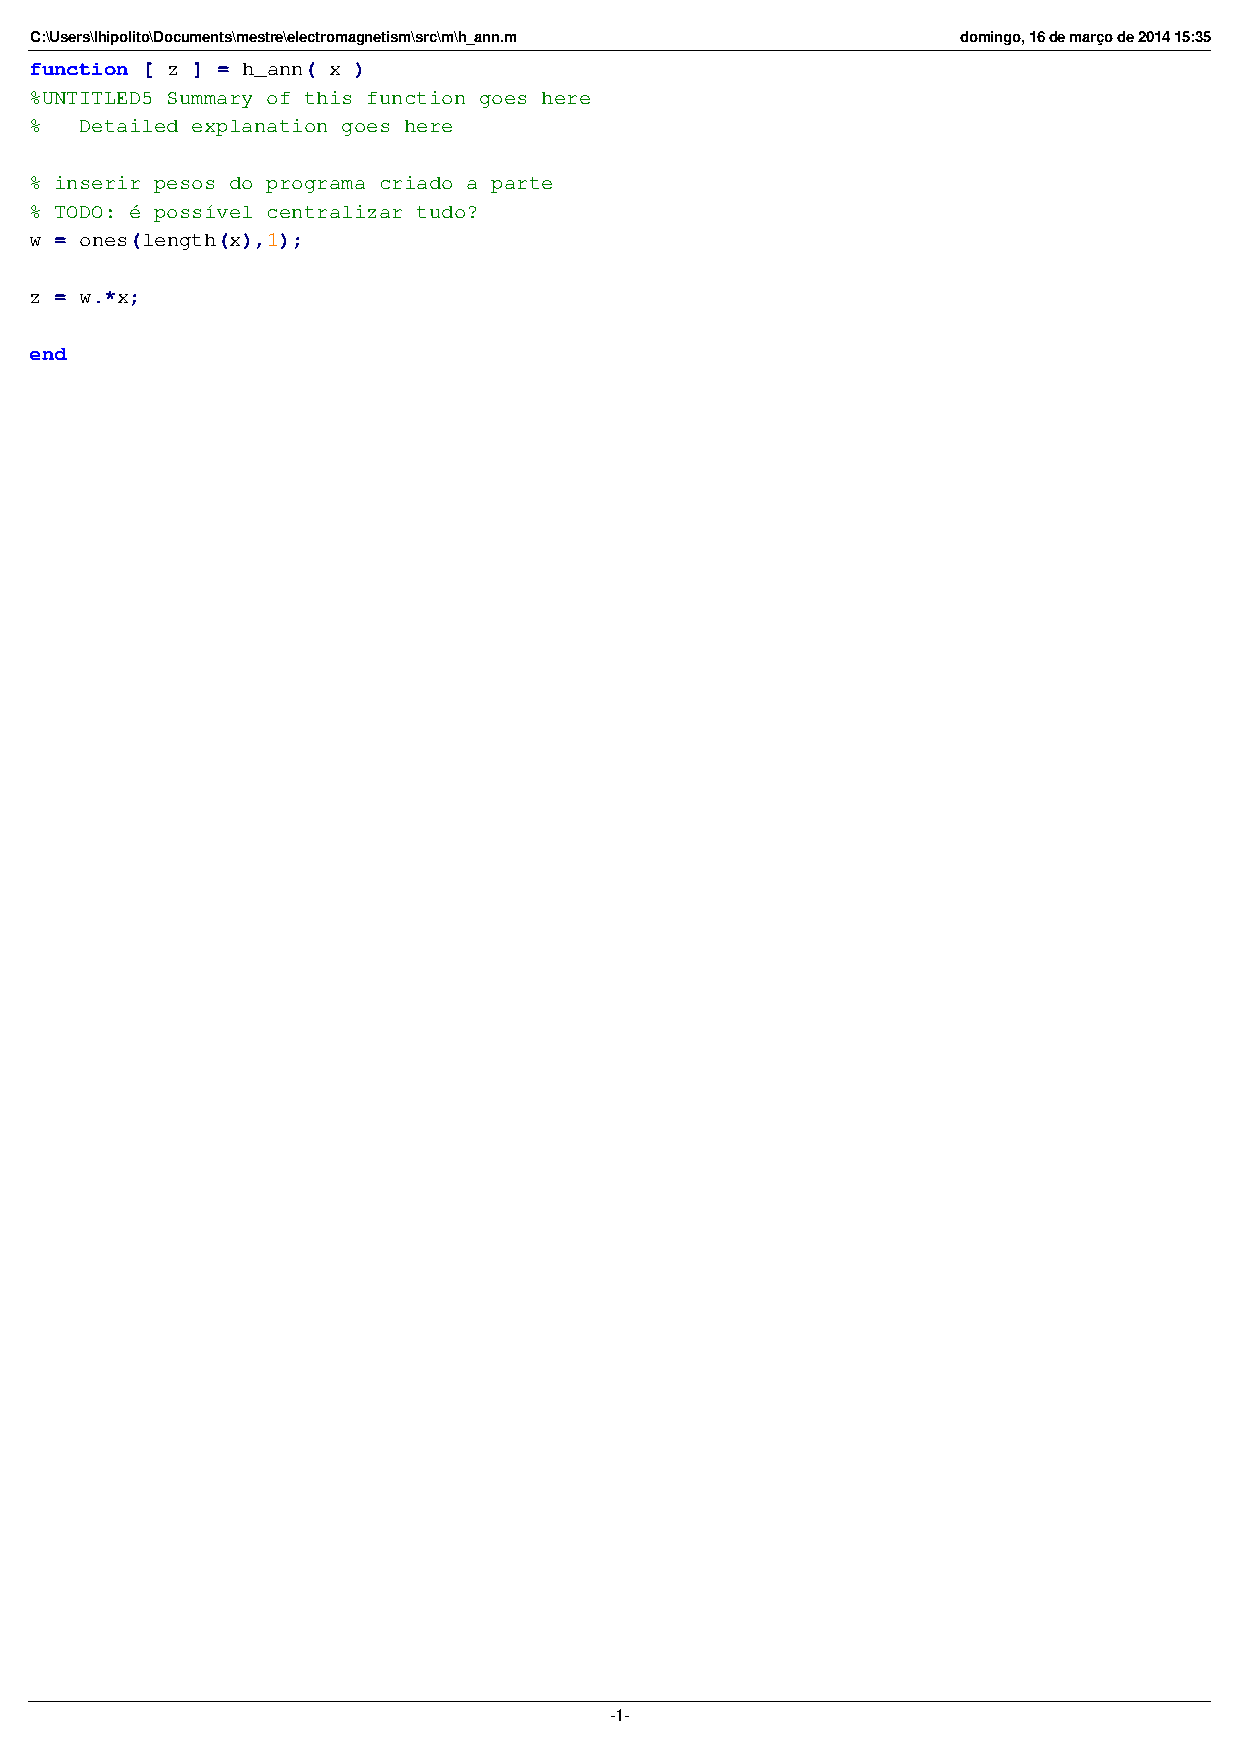
\includegraphics{h_ann.pdf}
	%\caption{Código}
	\label{h_ann}
\end{figure*}
\begin{figure*}
	\centering
	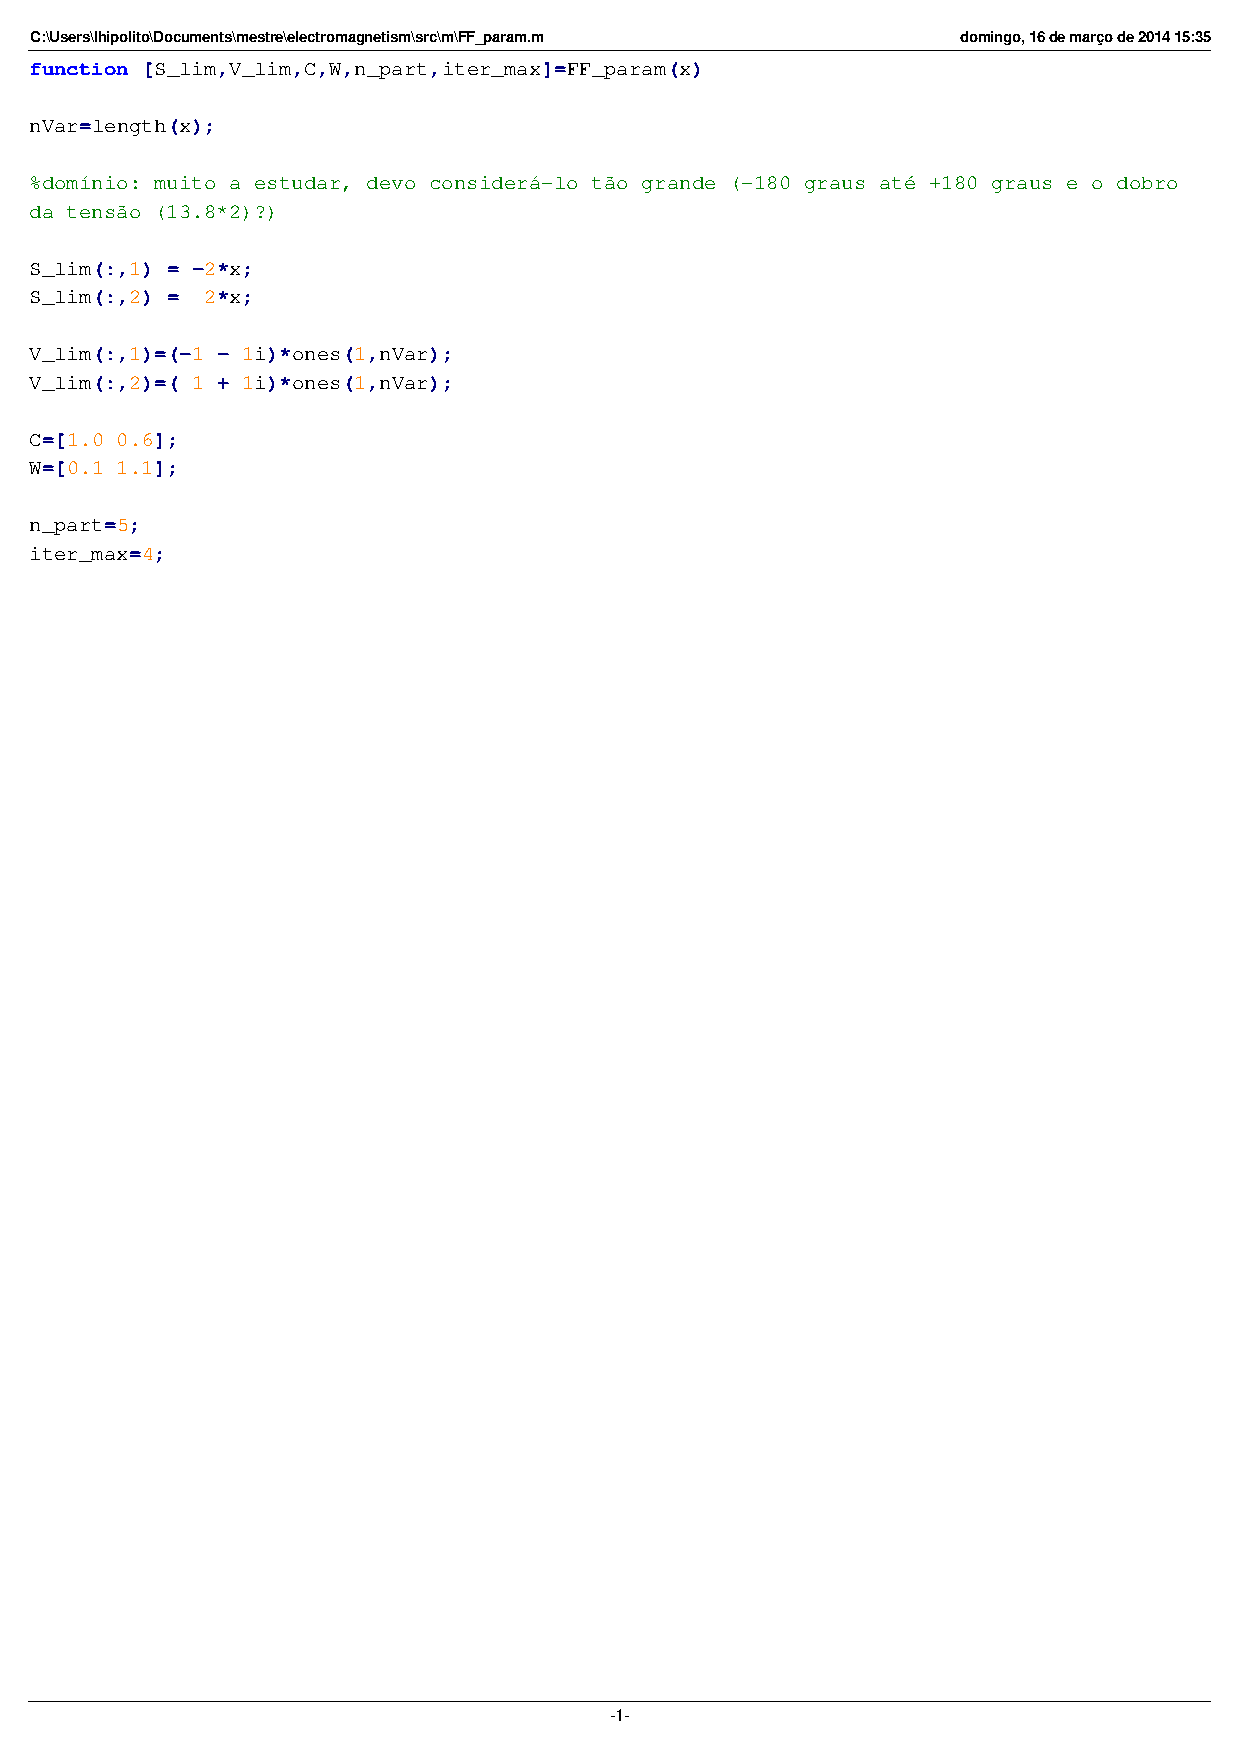
\includegraphics{FF_param.pdf}
	%\caption{Código}
	\label{FF_param}
\end{figure*}
\begin{figure*}
	\centering
	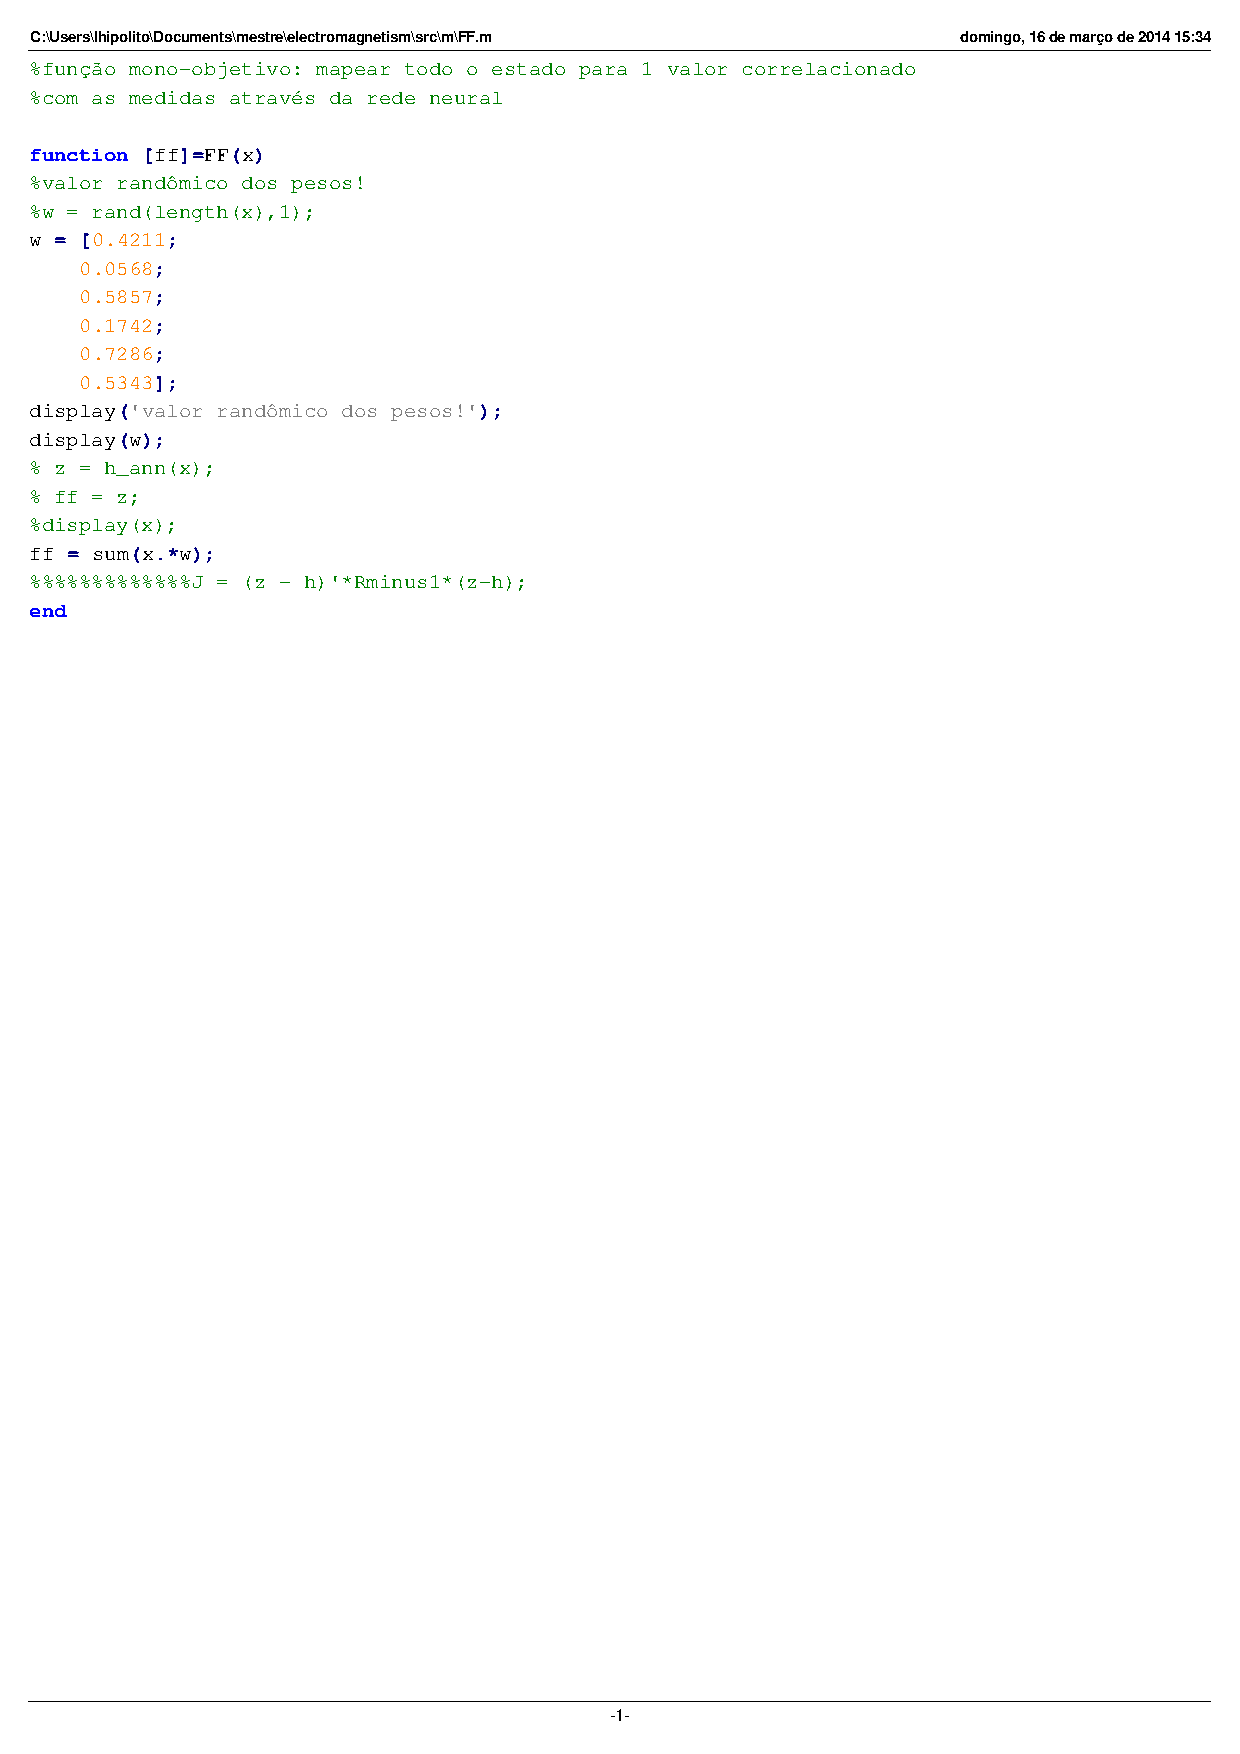
\includegraphics{FF.pdf}
	%\caption{Código}
	\label{FF}
\end{figure*}
\begin{figure*}
	\centering
	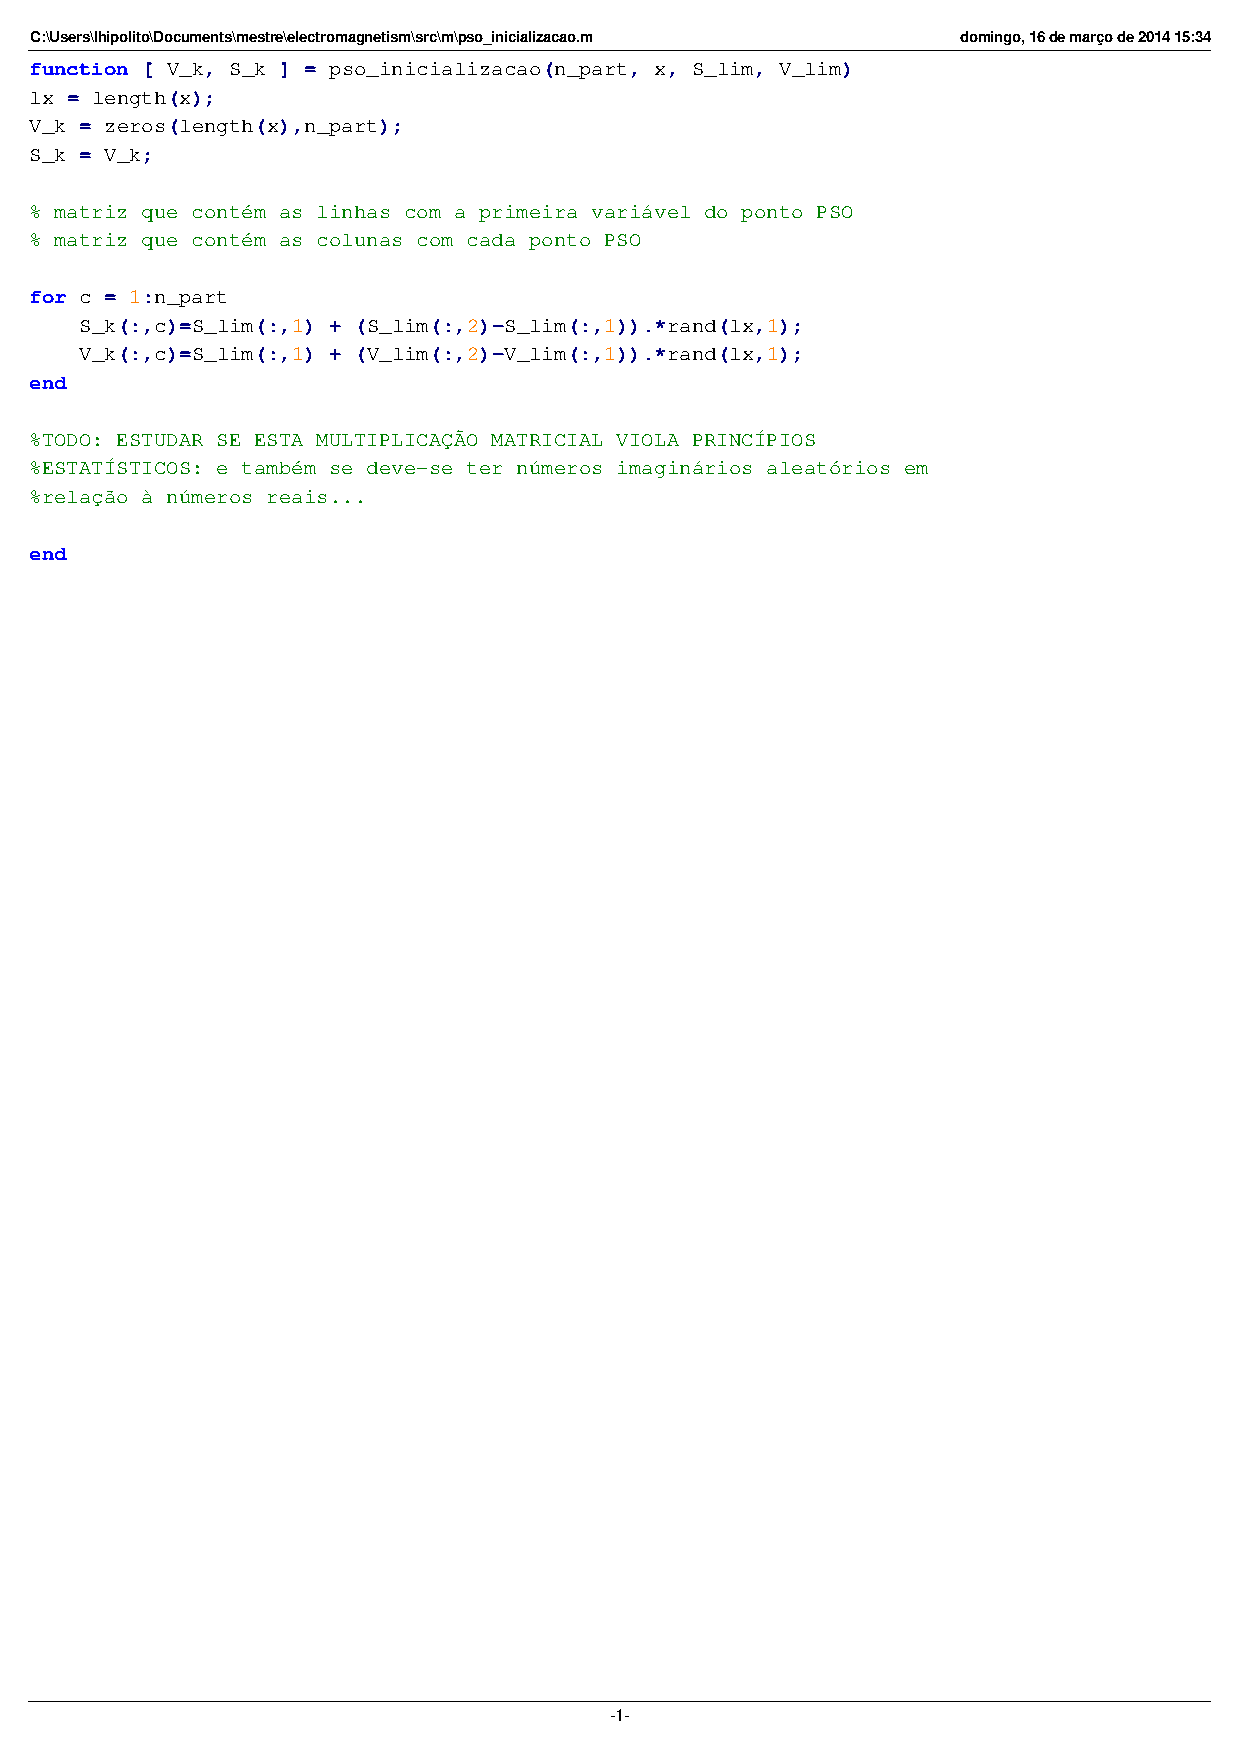
\includegraphics{pso_inicializacao.pdf}
	%\caption{Código}
	\label{pso_inicializacao}
\end{figure*}
\begin{figure*}
	\centering
	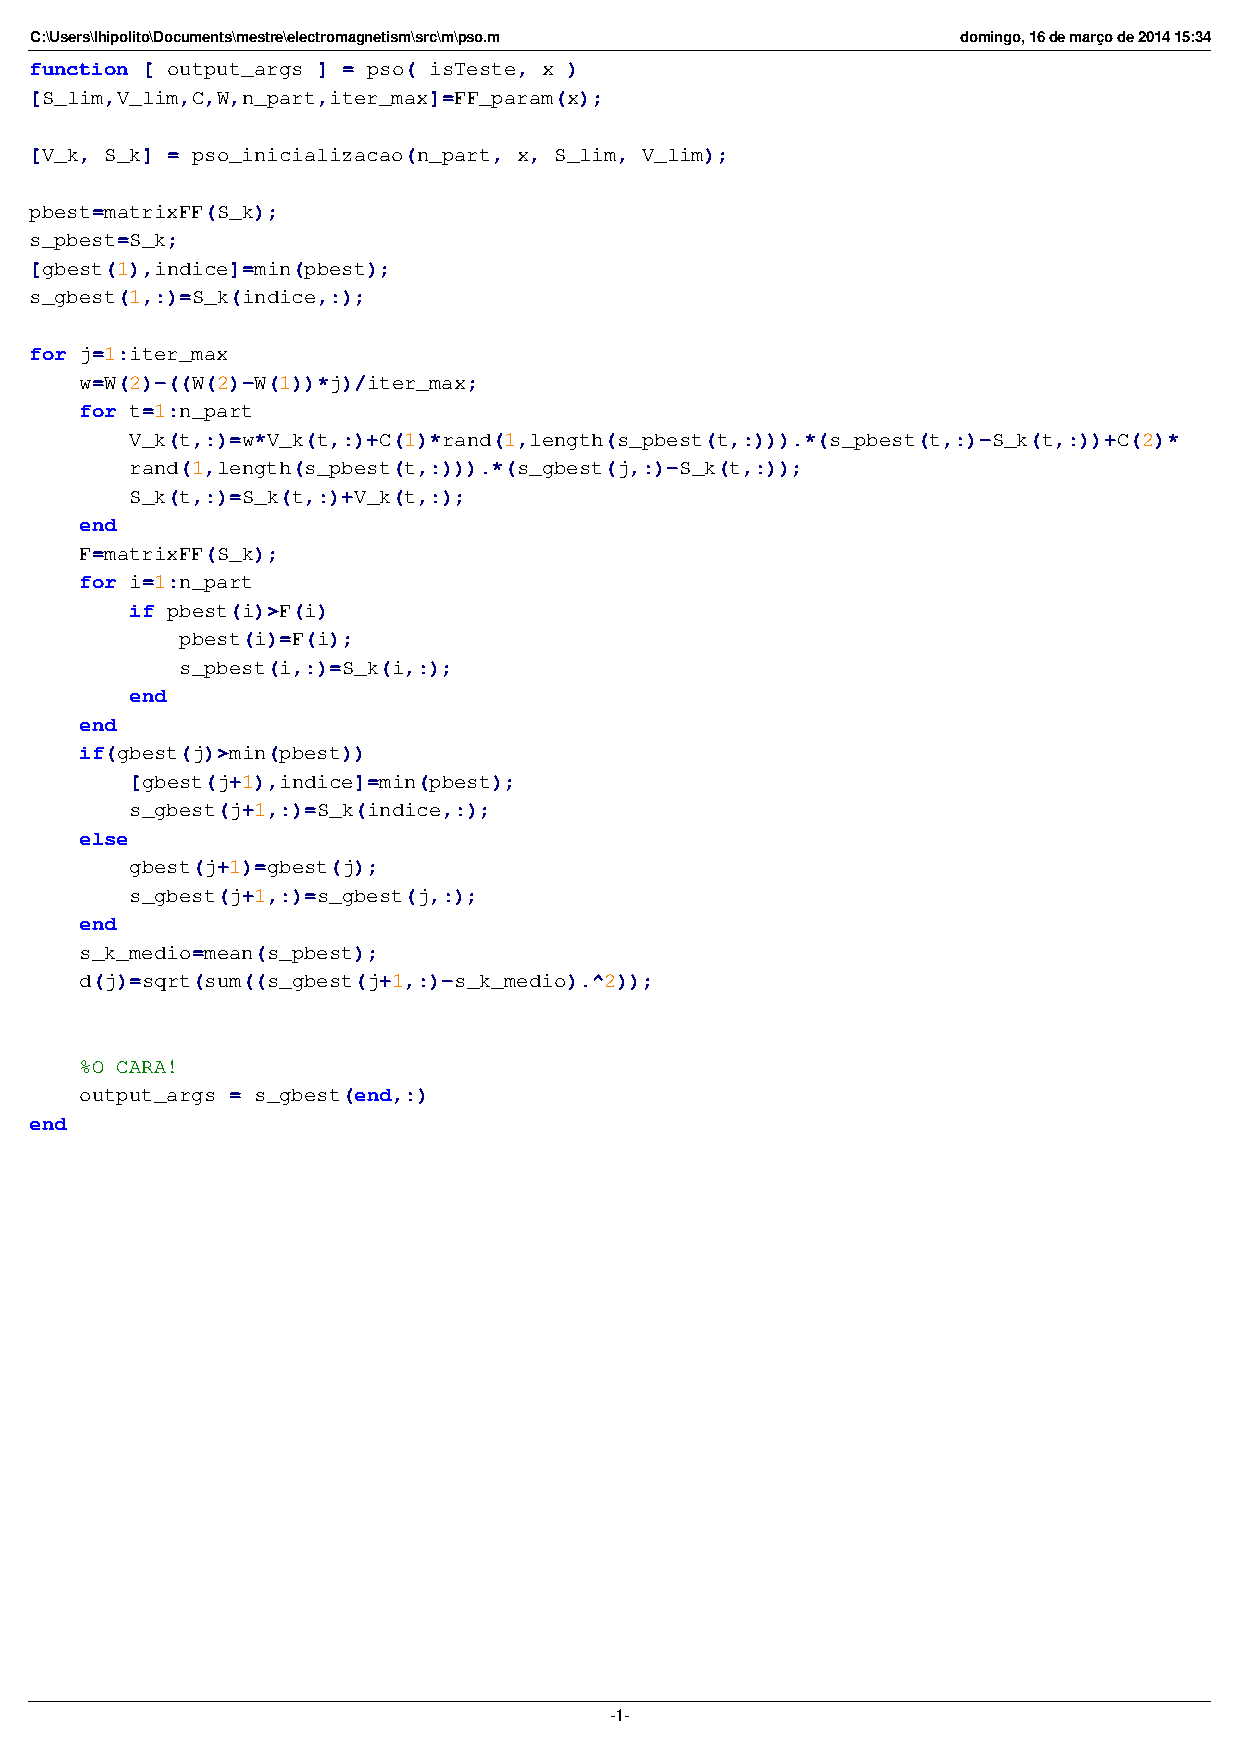
\includegraphics{pso.pdf}
	%\caption{Código}
	\label{pso}
\end{figure*}
\begin{figure*}
	\centering
	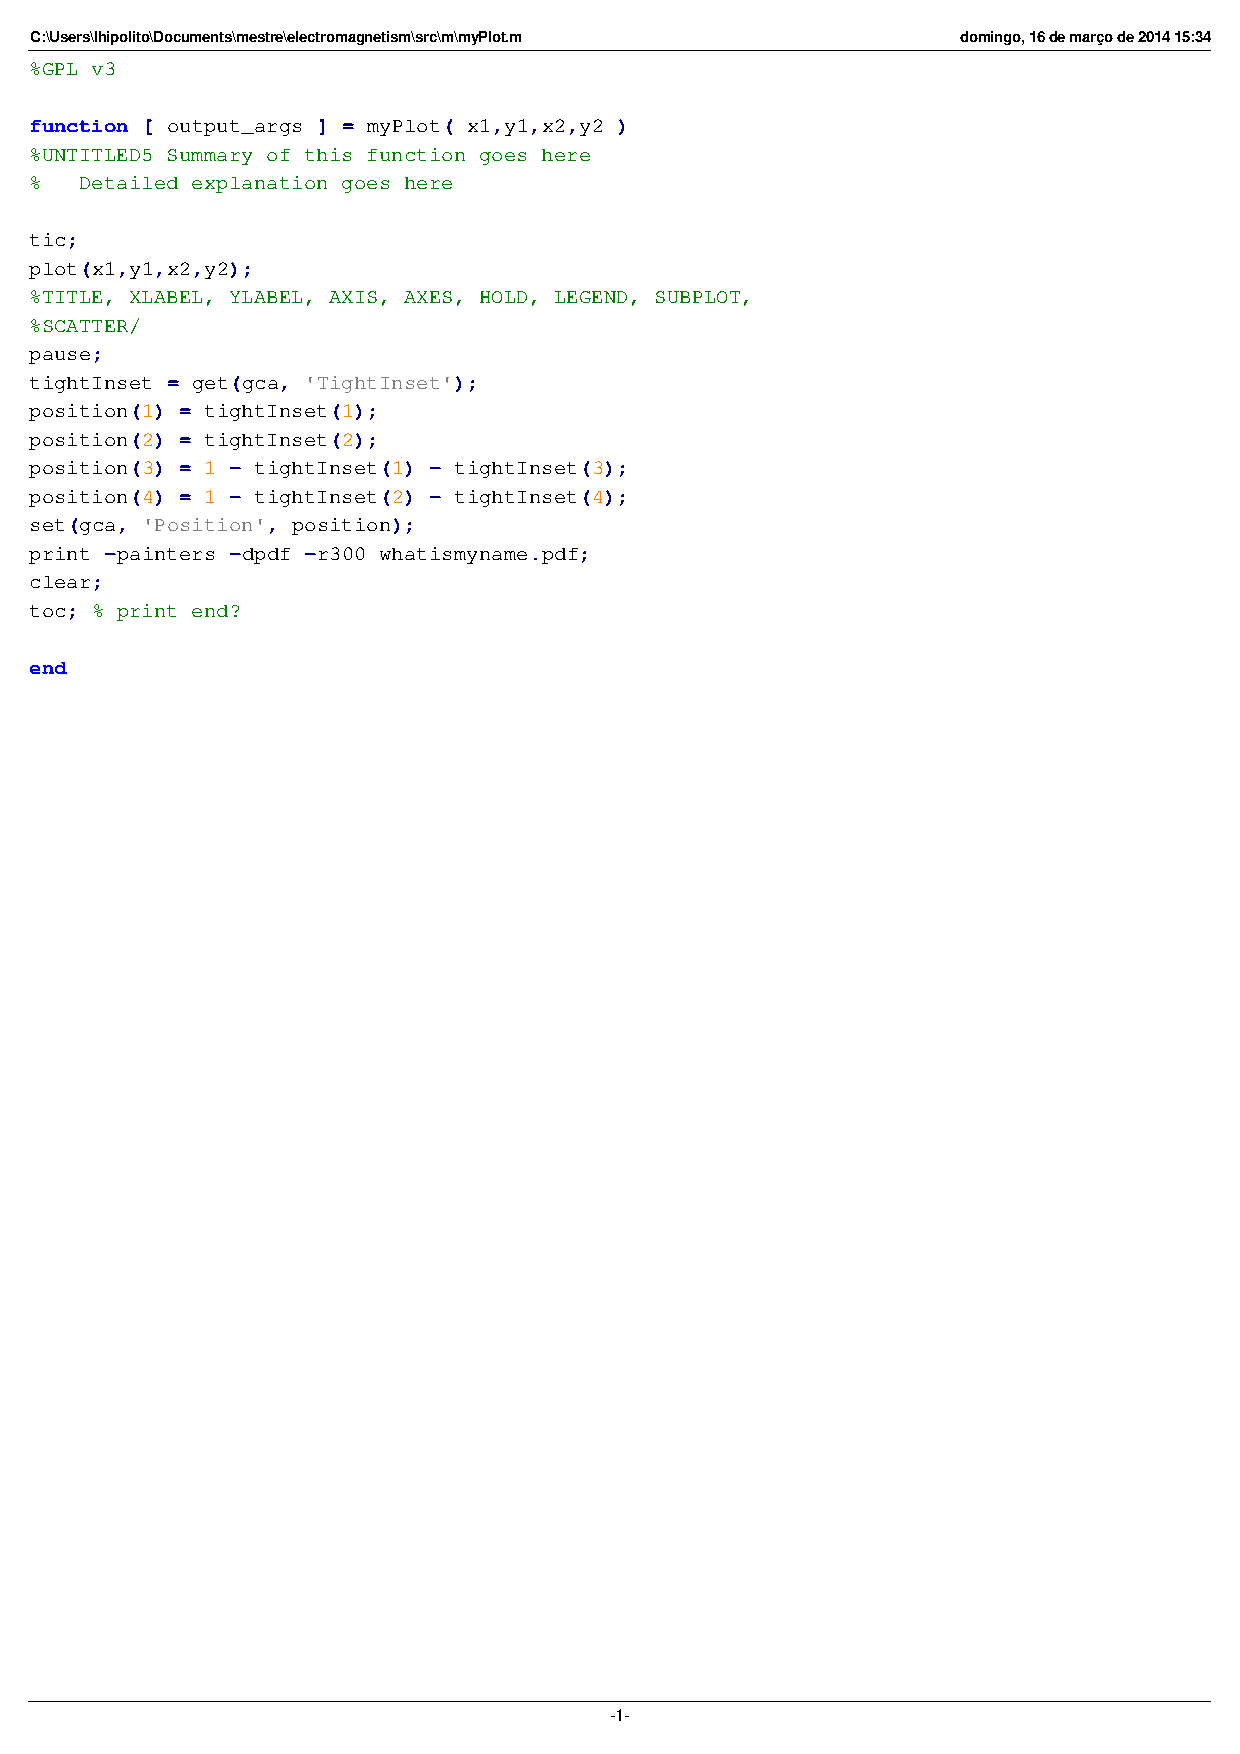
\includegraphics{myPlot.pdf}
	%\caption{Código}
	\label{myPlot}
\end{figure*}
\begin{figure*}
	\centering
	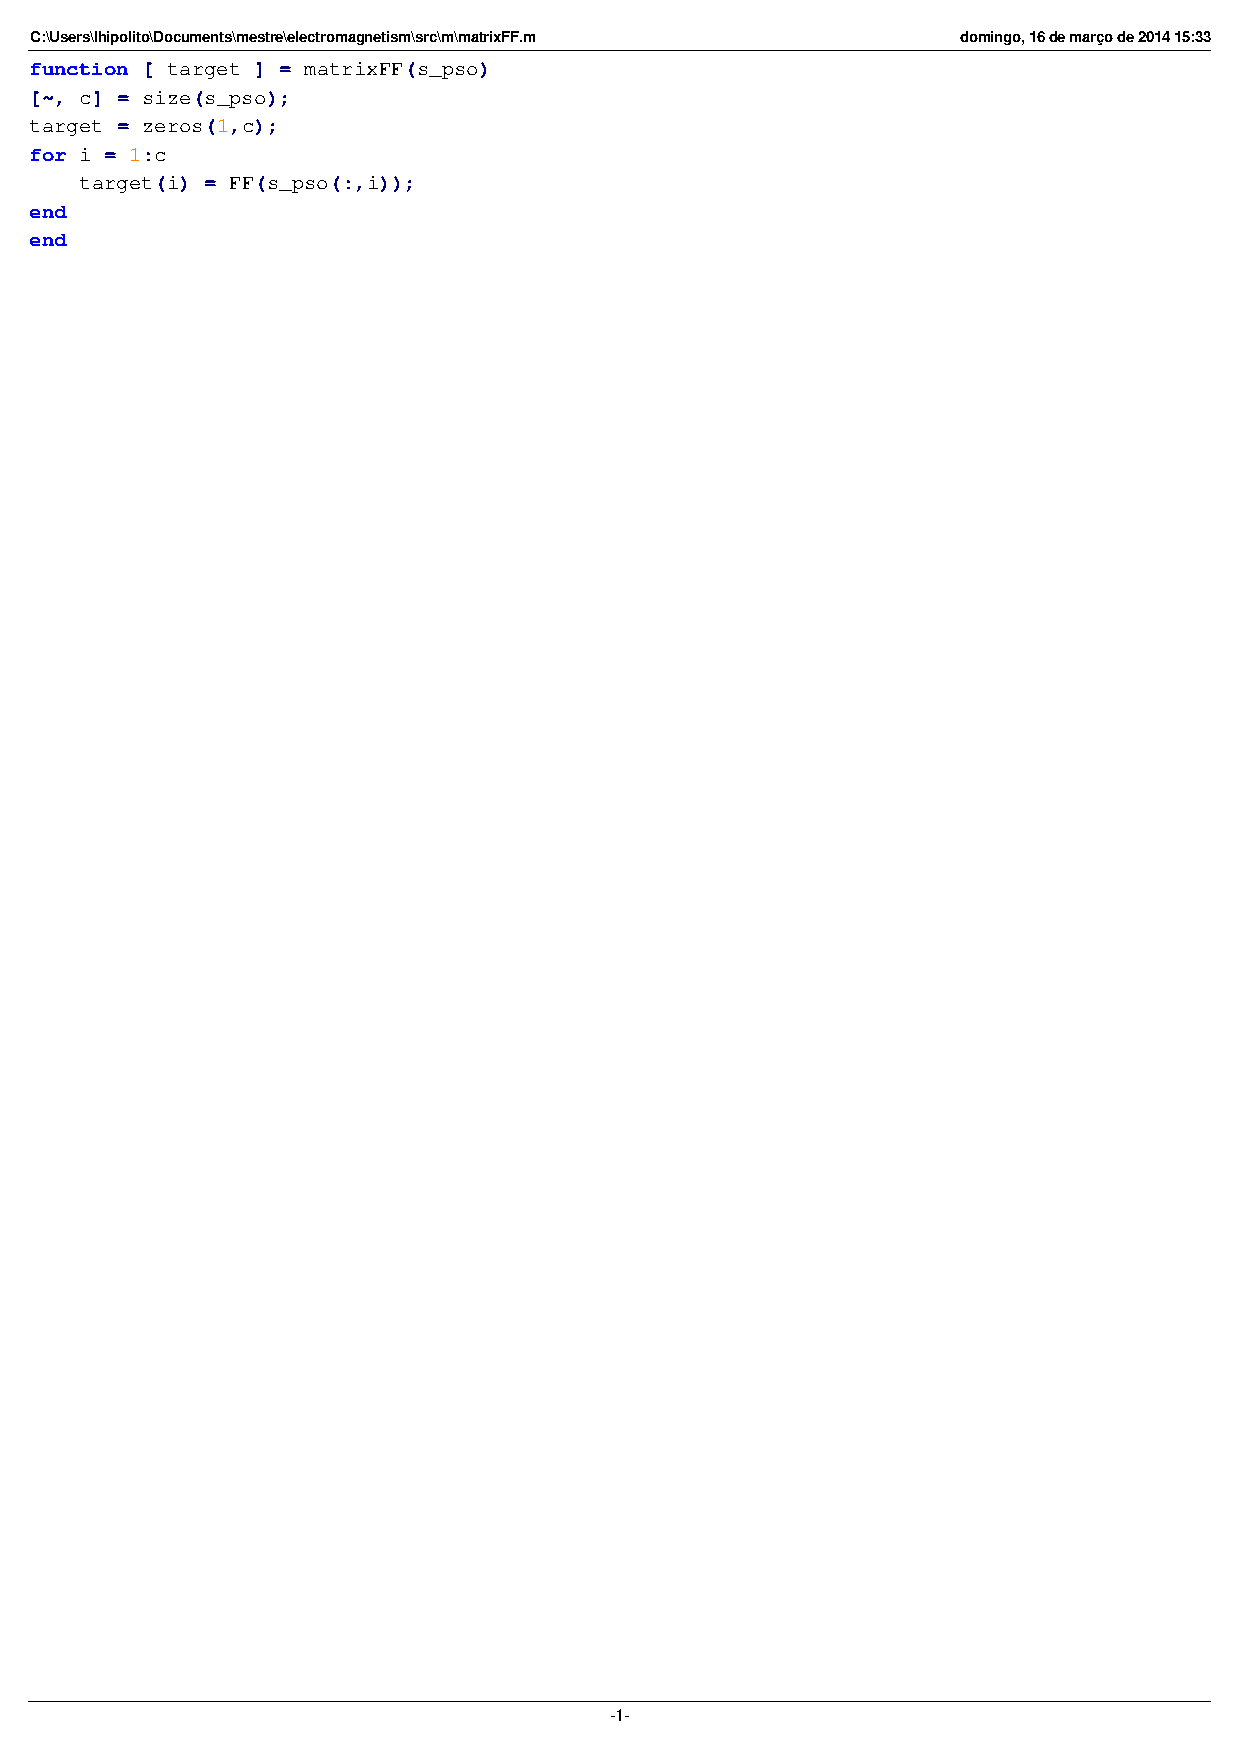
\includegraphics{matrixFF.pdf}
	%\caption{Código}
	\label{matrixFF}
\end{figure*}


% Can use something like this to put references on a page
% by themselves when using endfloat and the captionsoff option.
\ifCLASSOPTIONcaptionsoff
  \newpage
\fi

\bibliographystyle{ieeetran}
\bibliography{bib}

\begin{IEEEbiographynophoto}{Luiz Le Roy}
\'E um estudante do curso de mestrado da Pontif\'icia Universidade Cat\'olica de Minas Gerais.
\end{IEEEbiographynophoto}

% that's all folks
\end{document}
